

\tikzset{every picture/.style={line width=0.75pt}} %set default line width to 0.75pt        

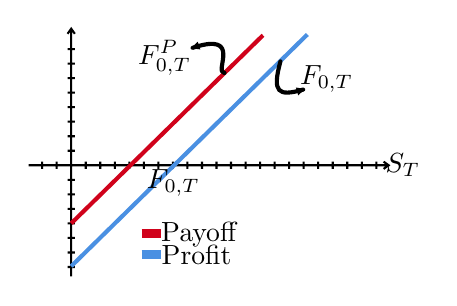
\begin{tikzpicture}[x=0.75pt,y=0.75pt,yscale=-0.35,xscale=0.35]
%uncomment if require: \path (0,363); %set diagram left start at 0, and has height of 363

%Shape: Axis 2D [id:dp37047505143526605] 
\draw  (14,196) -- (509.5,196)(72.5,8) -- (72.5,349) (502.5,191) -- (509.5,196) -- (502.5,201) (67.5,15) -- (72.5,8) -- (77.5,15) (92.5,191) -- (92.5,201)(112.5,191) -- (112.5,201)(132.5,191) -- (132.5,201)(152.5,191) -- (152.5,201)(172.5,191) -- (172.5,201)(192.5,191) -- (192.5,201)(212.5,191) -- (212.5,201)(232.5,191) -- (232.5,201)(252.5,191) -- (252.5,201)(272.5,191) -- (272.5,201)(292.5,191) -- (292.5,201)(312.5,191) -- (312.5,201)(332.5,191) -- (332.5,201)(352.5,191) -- (352.5,201)(372.5,191) -- (372.5,201)(392.5,191) -- (392.5,201)(412.5,191) -- (412.5,201)(432.5,191) -- (432.5,201)(452.5,191) -- (452.5,201)(472.5,191) -- (472.5,201)(492.5,191) -- (492.5,201)(52.5,191) -- (52.5,201)(32.5,191) -- (32.5,201)(67.5,176) -- (77.5,176)(67.5,156) -- (77.5,156)(67.5,136) -- (77.5,136)(67.5,116) -- (77.5,116)(67.5,96) -- (77.5,96)(67.5,76) -- (77.5,76)(67.5,56) -- (77.5,56)(67.5,36) -- (77.5,36)(67.5,216) -- (77.5,216)(67.5,236) -- (77.5,236)(67.5,256) -- (77.5,256)(67.5,276) -- (77.5,276)(67.5,296) -- (77.5,296)(67.5,316) -- (77.5,316)(67.5,336) -- (77.5,336) ;
\draw   ;
%Straight Lines [id:da30565410694888984] 
\draw [color={rgb, 255:red, 208; green, 2; blue, 27 }  ,draw opacity=1 ][line width=1.5]    (72.5,276) -- (336.5,17) ;


%Straight Lines [id:da2716512101716435] 
\draw [color={rgb, 255:red, 74; green, 144; blue, 226 }  ,draw opacity=1 ][line width=1.5]    (72.5,335) -- (397.5,16) ;


%Curve Lines [id:da4305252903013169] 
\draw [color={rgb, 255:red, 0; green, 0; blue, 0 }  ][line width=1.5] [line join = round][line cap = round]   (360.5,53) .. controls (348.8,95.9) and (357.06,101.73) .. (391.78,91.79) ;
\draw [shift={(394.5,91)}, rotate = 523.44] [fill={rgb, 255:red, 0; green, 0; blue, 0 }  ][line width=1.5] [line join = round][line cap = round] [draw opacity=0] (11.61,-5.58) -- (0,0) -- (11.61,5.58) -- cycle    ;

%Curve Lines [id:da29606513394571055] 
\draw [color={rgb, 255:red, 0; green, 0; blue, 0 }  ][line width=1.5] [line join = round][line cap = round]   (283.5,69) .. controls (267.71,69) and (309.65,11.17) .. (239.66,34.28) ;
\draw [shift={(237.5,35)}, rotate = 341.1] [fill={rgb, 255:red, 0; green, 0; blue, 0 }  ][line width=1.5] [line join = round][line cap = round] [draw opacity=0] (11.61,-5.58) -- (0,0) -- (11.61,5.58) -- cycle    ;

%Straight Lines [id:da27180621762709967] 
\draw [color={rgb, 255:red, 208; green, 2; blue, 27 }  ,draw opacity=1 ][line width=3]    (169.5,290) -- (196.5,290) ;


%Straight Lines [id:da47840375462275264] 
\draw [color={rgb, 255:red, 74; green, 144; blue, 226 }  ,draw opacity=1 ][line width=3]    (169.5,319) -- (196.5,319) ;




% Text Node
\draw (529,196) node  [align=left] {$\displaystyle S_{T}$};
% Text Node
\draw (424,77) node  [align=left] {$\displaystyle F_{0,T}$};
% Text Node
\draw (201,48) node  [align=left] {$\displaystyle F^{P}_{0,T}$};
% Text Node
\draw (213,220) node   {$F_{0,T}$};
% Text Node
\draw (248,291) node  [align=left] {Payoff};
% Text Node
\draw (245,320) node  [align=left] {Profit};


\end{tikzpicture}

